\documentclass[tikz,border=5pt]{standalone}
\usepackage[UTF8]{ctex}
\usepackage{amsmath,amssymb}
\usetikzlibrary{arrows.meta,calc,angles,quotes,decorations.pathmorphing}
\definecolor{ink}{HTML}{243447}\definecolor{blue}{HTML}{2765A2}
\definecolor{green}{HTML}{3F7D5B}\definecolor{red}{HTML}{B74739}
\tikzset{body/.style={draw=ink,thick},vec/.style={draw=blue,thick,-{Latex}},guide/.style={gray!65,dashed},dim/.style={ink,{Latex}-{Latex}},line cap=round,line join=round}
\begin{document}
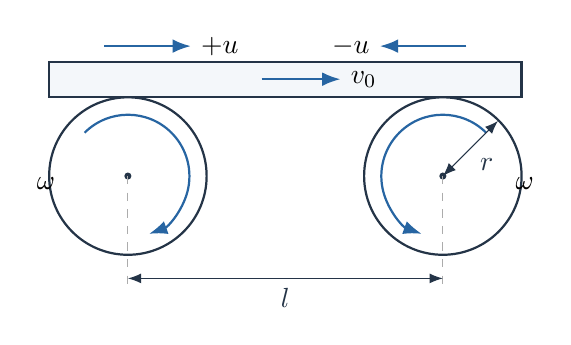
\begin{tikzpicture}
\draw[body,fill=blue!5](-1,1)--(5,1)--(5,1.45)--(-1,1.45)--cycle;
\draw[body](0,0)circle(1);\draw[body](4,0)circle(1);
\fill[ink](0,0)circle(.045);\fill[ink](4,0)circle(.045);
\draw[vec](-.3,1.65)--(.8,1.65)node[right]{$+u$};
\draw[vec](4.3,1.65)--(3.2,1.65)node[left]{$-u$};
\draw[vec](1.7,1.23)--(2.7,1.23)node[right]{$v_0$};
\draw[blue,-{Latex},thick](-.55,.55)arc(135:-70:.78);
\node[left]at(-.8,-.1){$\omega$};
\draw[blue,-{Latex},thick](4.55,.55)arc(45:250:.78);
\node[right]at(4.8,-.1){$\omega$};
\draw[dim](4,0)--(4.7,.7)node[midway,below right]{$r$};
\draw[guide](0,0)--(0,-1.45);\draw[guide](4,0)--(4,-1.45);
\draw[dim](0,-1.3)--(4,-1.3)node[midway,below]{$l$};
\end{tikzpicture}
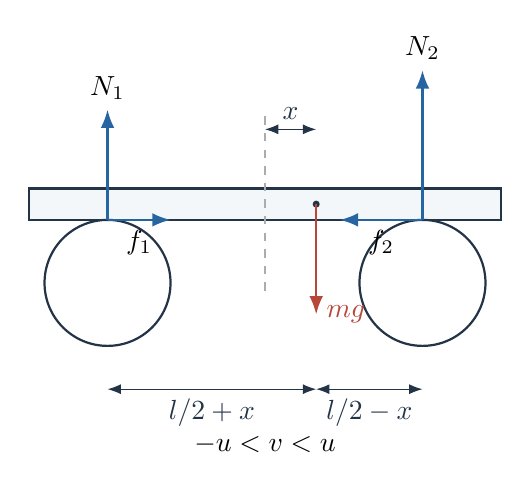
\begin{tikzpicture}
\draw[body,fill=blue!5](-1,1)--(5,1)--(5,1.4)--(-1,1.4)--cycle;
\draw[body](0,.2)circle(.8);\draw[body](4,.2)circle(.8);
\draw[guide](2,.1)--(2,2.4);\fill[ink](2.65,1.2)circle(.045);
\draw[vec](0,1)--(0,2.4)node[above]{$N_1$};
\draw[vec](4,1)--(4,2.9)node[above]{$N_2$};
\draw[red,thick,-{Latex}](2.65,1.2)--(2.65,-.2)node[right]{$mg$};
\draw[vec](0,1)--(.8,1)node[midway,below]{$f_1$};
\draw[vec](4,1)--(2.95,1)node[midway,below]{$f_2$};
\draw[dim](2,2.15)--(2.65,2.15)node[midway,above]{$x$};
\draw[dim](0,-1.15)--(2.65,-1.15)node[midway,below]{$l/2+x$};
\draw[dim](2.65,-1.15)--(4,-1.15)node[midway,below]{$l/2-x$};
\node at(2,-1.85){$-u<v<u$};
\end{tikzpicture}
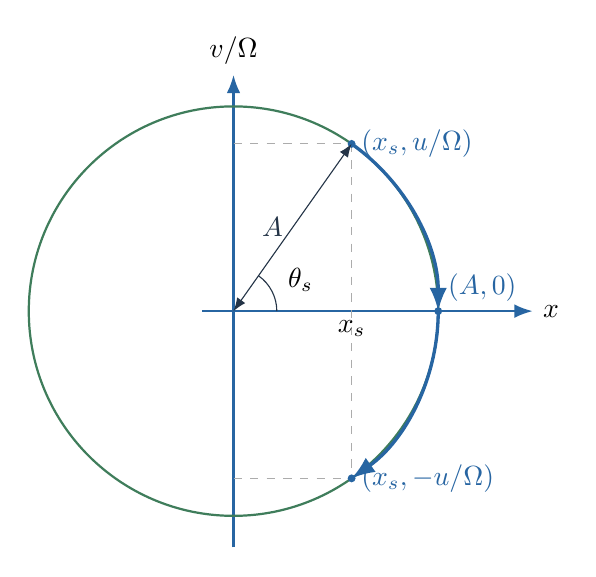
\begin{tikzpicture}
\draw[vec](-.4,0)--(3.8,0)node[right]{$x$};
\draw[vec](0,-3)--(0,3)node[above]{$v/\Omega$};
\draw[green,thick](0,0)circle(2.6);
\draw[blue,very thick,-{Latex}](1.5,2.124)arc(54.76:0:2.6);
\draw[blue,very thick,-{Latex}](2.6,0)arc(0:-54.76:2.6);
\draw[guide](1.5,2.124)--(1.5,-2.124);
\draw[guide](0,2.124)--(1.5,2.124);\draw[guide](0,-2.124)--(1.5,-2.124);
\fill[blue](1.5,2.124)circle(.05)node[right]{$(x_s,u/\Omega)$};
\fill[blue](1.5,-2.124)circle(.05)node[right]{$(x_s,-u/\Omega)$};
\fill[blue](2.6,0)circle(.05)node[above right]{$(A,0)$};
\draw[dim](0,0)--(1.5,2.124)node[midway,left]{$A$};
\draw[ink](.55,0)arc(0:54.76:.55);\node at(.85,.4){$\theta_s$};
\node[below]at(1.5,0){$x_s$};
\end{tikzpicture}
\begin{tikzpicture}
\draw[body](0,0)--(9,0);
\fill[blue](0,0)circle(.05)node[below]{$0$};
\fill[blue](3,0)circle(.05)node[below]{$x_s$};
\fill[green](6,0)circle(.05)node[below]{$A$};
\draw[vec](0,.7)--(3,.7)node[midway,above]{匀减速 $v_0\to u$};
\draw[vec](3,1.9)--(6,1.9)node[midway,above]{简谐去程};
\draw[vec](6,3)--(3,3)node[midway,above]{简谐返程 $0\to-u$};
\draw[vec](3,-1.2)--(0,-1.2)node[midway,below]{匀速 $v=-u$};
\begin{scope}[shift={(8,1.5)}]
\draw[body,fill=blue!5](-1.2,0)rectangle(1.2,.3);
\draw[vec](-.8,0)--(-.15,0)node[midway,below]{$\mu N_1$};
\draw[red,thick,-{Latex}](.8,0)--(.15,0)node[midway,above]{$f_{2s}$};
\node at(0,1){$|f_{2s}|=\mu N_1\leq\mu N_2$};
\end{scope}
\end{tikzpicture}
\end{document}
